\documentclass[10pt]{article}\usepackage[]{graphicx}\usepackage[]{color}
%% maxwidth is the original width if it is less than linewidth
%% otherwise use linewidth (to make sure the graphics do not exceed the margin)
\makeatletter
\def\maxwidth{ %
  \ifdim\Gin@nat@width>\linewidth
    \linewidth
  \else
    \Gin@nat@width
  \fi
}
\makeatother

\usepackage{Sweavel}


\usepackage{hyperref}
\usepackage{url}
\usepackage[a4paper]{geometry}
\usepackage{a4wide}
\usepackage{float}
\usepackage[english]{babel}
\usepackage[utf8]{inputenc}
\usepackage{csquotes}
\usepackage{amsmath}
\usepackage{amssymb}
\usepackage{xspace}
\usepackage[numbers]{natbib}
\bibliographystyle{unsrtnat}
\usepackage{subcaption}
\usepackage[font={small}]{caption}
\usepackage{booktabs}
\usepackage{listings}
\usepackage{cleveref}
\usepackage{lipsum}
\usepackage{graphicx}
\usepackage{epstopdf}
\graphicspath{{../figures/}}
\epstopdfsetup{outdir=./}
\newcommand{\approxtext}[1]{\ensuremath{\stackrel{\text{#1}}{=}}}
\newcommand{\matr}[1]{\mathbf{#1}}
\newcommand{\partt}[2]{\ensuremath{\dfrac{\partial {#1}}{\partial {#2}}}}
\renewcommand{\d}[1]{\ensuremath{\operatorname{d}\!{#1}}} % non-italized differentials
\newcommand{\h}[0]{\ensuremath{\hbar}} % hbar
\def\changemargin#1#2{\list{}{\rightmargin#2\leftmargin#1}\item[]}
\let\endchangemargin=\endlist 
\usepackage{amsthm}
\theoremstyle{plain}
\renewcommand{\theequation}{\thesection.\arabic{equation}}
\def\changemargin#1#2{\list{}{\rightmargin#2\leftmargin#1}\item[]}
\let\endchangemargin=\endlist    
\usepackage{xcolor}
\definecolor{Red}{rgb}{0.7,0,0}
\definecolor{Blue}{rgb}{0,0,0.8}
\usepackage{verbatim}
\def\changemargin#1#2{\list{}{\rightmargin#2\leftmargin#1}\item[]}
\let\endchangemargin=\endlist
\addtolength{\oddsidemargin}{-.35in}
\addtolength{\evensidemargin}{-.35in}
\addtolength{\textwidth}{.7in}
\usepackage{multicol}

% Stephen's stuff
\newcommand{\R}{\texttt{R}}
\newcommand{\Rfunction}[1]{{\texttt{#1}}}
\newcommand{\Robject}[1]{{\texttt{#1}}}
\newcommand{\Rpackage}[1]{{\mbox{\normalfont\textsf{#1}}}}
\usepackage{xcolor}
\definecolor{Red}{rgb}{0.7,0,0}
\definecolor{Blue}{rgb}{0,0,0.8}
\hypersetup{%
pdfusetitle,
bookmarks = {true},
bookmarksnumbered = {true},
bookmarksopen = {true},
bookmarksopenlevel = 2,
unicode = {true},
breaklinks = {false},
hyperindex = {true},
colorlinks = {true},
linktocpage = {true},
plainpages = {false},
linkcolor = {Blue},
citecolor = {Blue},
urlcolor = {Red},
pdfstartview = {Fit},
pdfpagemode = {UseOutlines},
pdfview = {XYZ null null null}
}
%% Listings
\lstset{ 
language=R,                     % the language of the code
basicstyle=\footnotesize,       % the size of the fonts that are used for the code
numbers=left,                   % where to put the line-numbers
numberstyle=\tiny\color{gray},  % the style that is used for the line-numbers
stepnumber=1,                   % the step between two line-numbers. If it's 1, each line will be numbered
numbersep=5pt,                  % how far the line-numbers are from the code
backgroundcolor=\color{white},  % choose the background color. You must add \usepackage{color}
showspaces=false,               % show spaces adding particular underscores
showstringspaces=false,         % underline spaces within strings
showtabs=false,                 % show tabs within strings adding particular underscores
rulecolor=\color{black},        % if not set, the frame-color may be changed on line-breaks within not-black text (e.g. commens (green here))
tabsize=2,                      % sets default tabsize to 2 spaces
captionpos=b,                   % sets the caption-position to bottom
breaklines=true,                % sets automatic line breaking
breakatwhitespace=false,        % sets if automatic breaks should only happen at whitespace
title=\lstname,                 % show the filename of files included with \lstinputlisting;
% also try caption instead of title
keywordstyle=\color{Blue},      % keyword style
commentstyle=\color{orange},    % comment style
stringstyle=\color{Red},        % string literal style
% escapeinside={\%*}{*)},         % if you want to add a comment within your code
% escapeinside={\%}{)},
morekeywords={*,...}            % if you want to add more keywords to the set
} 

%%% Document specific
\newcommand{\course}{Computational Neuroscience}
\newcommand{\ass}{1}
\newcommand{\term}{Lent term 2017}
  

%\bibliography{pga1}

%%% Title page
\title{
  \bf \course: Assignment \ass \\[1em]
  \small{University of Cambridge}
}

\author{Henrik Åhl}
\date{\today}
\renewcommand{\textfraction}{0.05}
\renewcommand{\topfraction}{0.8}
\renewcommand{\bottomfraction}{0.8}
\renewcommand{\floatpagefraction}{0.75}

%%% Actual document
\begin{document}
\date{\today}
\maketitle
\setcounter{page}{1}
\setcounter{section}{1}


% \date{\today}
\maketitle
% \begin{abstract}
% 	{\bf 
% 		%\begin{changemargin}{-.8cm}{-.8cm}
% 		This is an abstract abstract.
% 	}
% \end{abstract}
\begin{multicols*}{2}
	\section*{Preface}
	This is an assignment report in connection to the \textit{\course}
	module in the Computational Biology course at the University of Cambridge,
	\term. All related code is as of \date{\today} available through a
	Github repository by contacting \href{mailto:hpa22@cam.ac.uk}{hpa22@cam.ac.uk}.
	\section*{Exercises}
	\paragraph*{1}
	
	The four parameters $v, u, I_e$ and $\epsilon$ denote the neuron membrane voltage, a recovery variable, an external stimulus input current, and a time-scale parameter respectively. We plot the nullclines in \cref{fig:nullclines}. Implementing Newton's method to find the roots of the composite equation $v^3 + v + 1 = 0$, we find that they are given by $0.5u = v~=~$-0.6823278, -0.6823278$i$ and 0.6823278$i$ for $I_e = -1$, and $u = v = 0$ and $v = \pm i, u = \pm 2i$ for $I_e = 0$. Observing the nullcline figures, we see that this appears visually likely as well. 
	
\begin{Schunk}
\begin{figure}[H]

{\centering 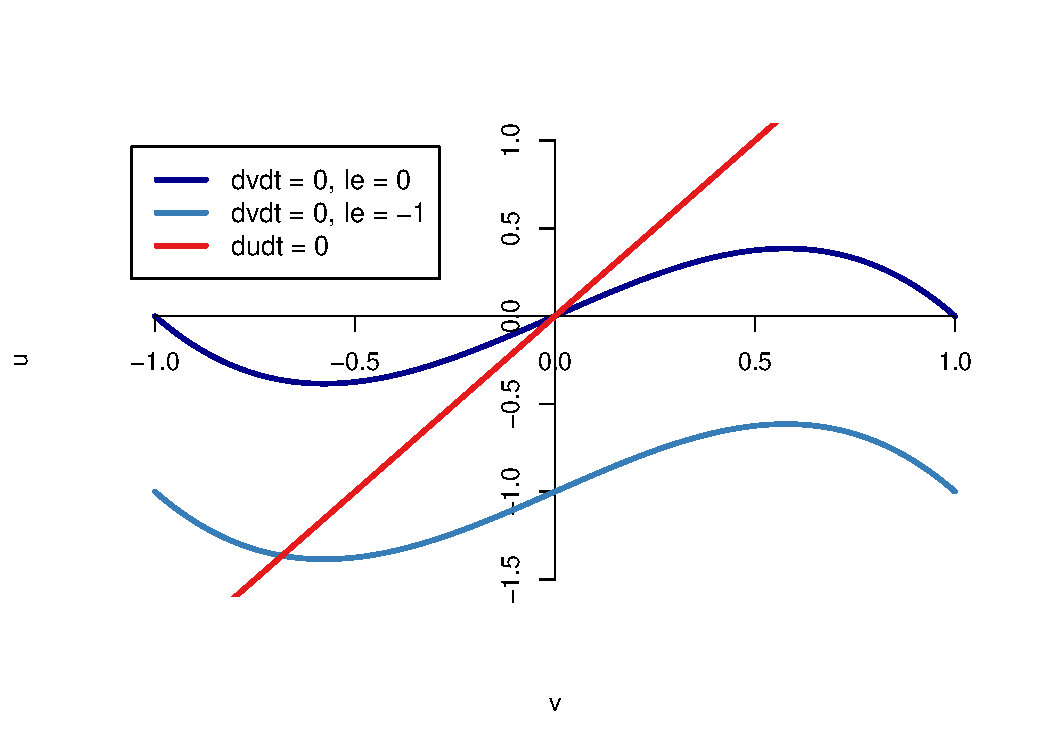
\includegraphics[width=\maxwidth]{../figures/twocolumn-nullclines-1} 

}

\caption[Nullclines of the system plotted as functions of $u$]{Nullclines of the system plotted as functions of $u$.}\label{fig:nullclines}
\end{figure}
\end{Schunk}
	
	
\begin{Schunk}
\begin{figure}[H]

{\centering \includegraphics[width=\maxwidth]{../figures/twocolumn-trajectories_i0-1} 

}

\caption{Trajectories for $\epsilon = \{0.1, 0.3, 1.0\}$ respectively, with $I_e = 0$. Note how all trajectories diverge from the unstable fixpoint at the origin, and how the eccentricity of the phase diagram changes with altered $\epsilon$.}\label{fig:trajectories.i0}
\end{figure}
\end{Schunk}
	~
\begin{Schunk}
\begin{figure}[H]

{\centering 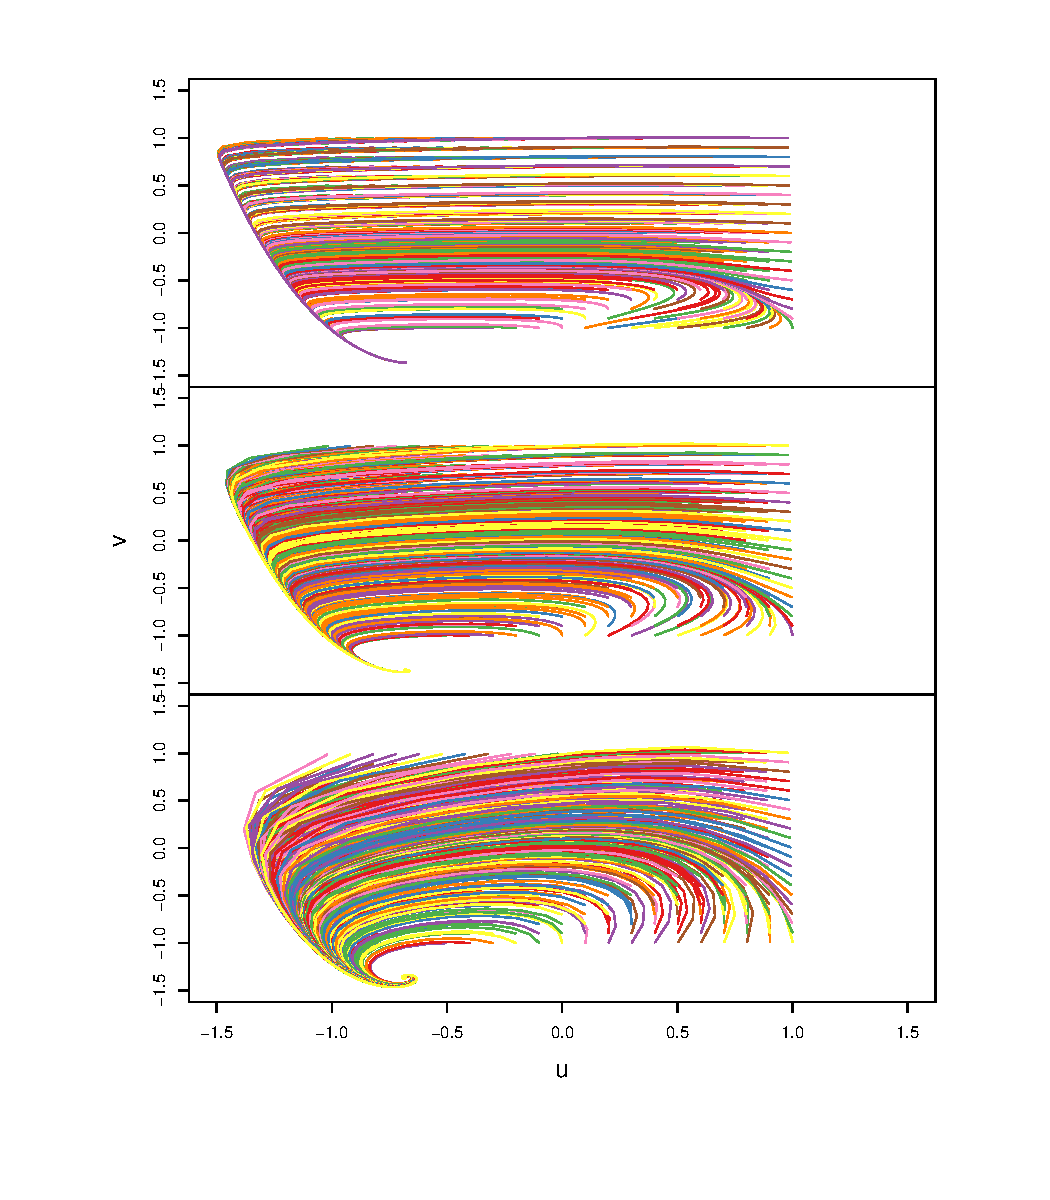
\includegraphics[width=\maxwidth]{../figures/twocolumn-trajectories_i-1-1} 

}

\caption{Similar to \cref{fig:trajectories.i0}, but for $I_e = -1$. Note how all trajectories converge to the same point, and again, how the eccentricity changes with $\epsilon$.}\label{fig:trajectories.i-1}
\end{figure}
\end{Schunk}
	
	%%%%%%%%%%%%%%%%%%%%%%%%%%%%%%%%%%%%%%%%%%%%%%%%%%%%%%%%
	%%% Question 1b
	%%%%%%%%%%%%%%%%%%%%%%%%%%%%%%%%%%%%%%%%%%%%%%%%%%%%%%%%
	When analysing the stability of the system, we consider the Jacobian matrix we get from our equations:
	\begin{align}
	\matr J =  \left(
  	\begin{matrix}
      1 - 3v^2  & -1                   \\
      \epsilon  & \dfrac{\epsilon}{2}
    \end{matrix}
    \right)
	\end{align}
	
	For stability we require, as before, that 
	\begin{align}
  	0 &= v(1-v^2) -u + I_e \\
  	0 &= \epsilon (v - \dfrac{u}{2})
	\end{align}
	as previously, which again gives us $u = 2v$, but also $I_e = v(1 + v^2)$.
	
	From the Hopf bifurcation theorem, we require $Tr(\matr J) = 0$, and as a results also $det(\matr J) > 0$. Investigating this we get that 
	\begin{align}
	  Tr(\matr J) &= 1-3v^2 - \dfrac{\epsilon}{2} = 0 \Leftrightarrow 1 - 3v^2 = \dfrac{\epsilon}{2} \\
	  &\Rightarrow v = \pm \sqrt{\dfrac{1 - \dfrac{\epsilon}{2}}{3}} \\
	  det(\matr J) &= \epsilon - \dfrac{\epsilon}{2}(1-3v^2) > 0 
	\end{align}
	from where it follows that 
	\begin{align}
	  \epsilon (\epsilon + 3) > 0 \Rightarrow \epsilon < -3 \lor \epsilon > 0.
	\end{align}
	Imposing the physical requirement of positive $\epsilon$, we see that we simply require the constant to be non-zero. Considering $I_e$ we find from above that 
	\begin{align}
	  I_e (\epsilon) \lessgtr \pm \sqrt{\dfrac{1 - \dfrac{\epsilon}{2}}{3}}\left( \dfrac{4}{3} - \dfrac{\epsilon}{6} \right)
	\end{align}
	where we also see that we require $\epsilon \leq 2$ for a real-valued solution.
	Plotting this region, we get the one seen in \cref{fig:Ie}.
	
\begin{Schunk}
\begin{figure}[H]

{\centering 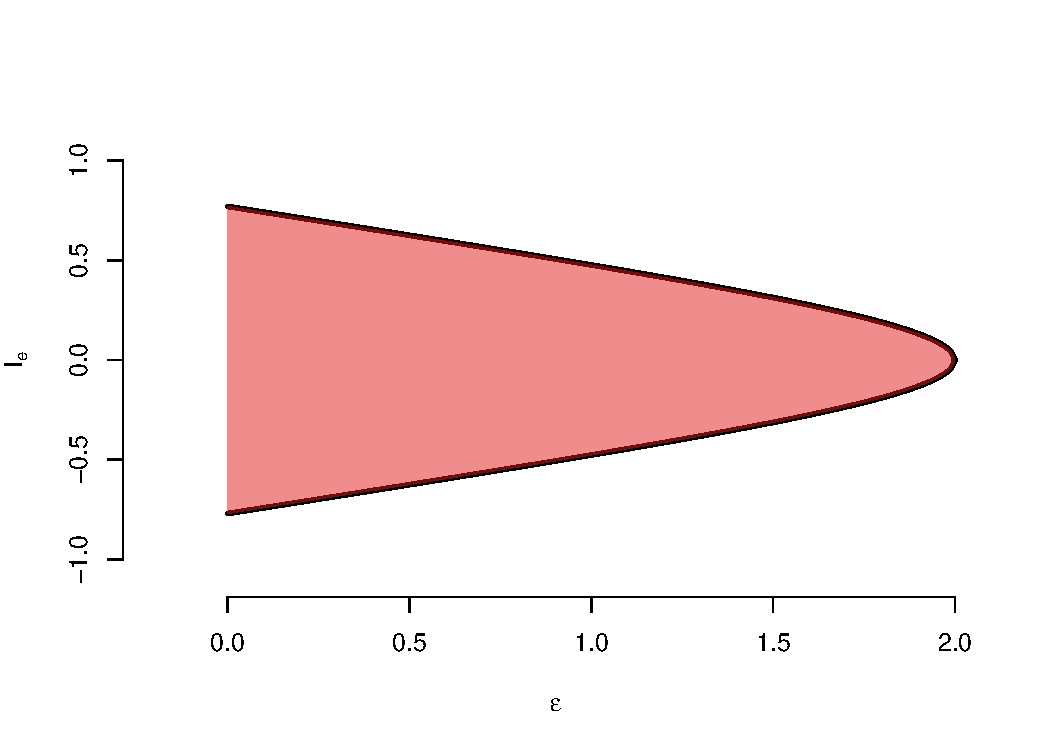
\includegraphics[width=\maxwidth]{../figures/twocolumn-Ie-1} 

}

\caption[Parameter area giving rise to oscillation in thr system]{Parameter area giving rise to oscillation in thr system. Note how we indeed for all cases when $I_e = 0$ can expect oscillations for our choices of $\epsilon$, but for none of the cases when $I_e = -1$.}\label{fig:Ie}
\end{figure}
\end{Schunk}
	
	\paragraph*{2}
	Using a perceptron with a given bias node, we implement the three rules to classify our input data. In all our comparisons we use 10 inputs (and weights) aside of the bias. When not comparing learning time, we iterate the perceptron and delta rules 10 times the number of patterns contained in the training data set. We also consistently use a learning rate of 0.1 and replicate each setting 200 times for statistical purposes. 
	
	When using a linear input function for the delta rule, it reduces to the perceptron rule. We therefore instead of a linear input function modify our inputs by parsing them through the error function, which simply increases the sign sensitivity of the data. However, the effect this gives is to simply this only corresponds to changing the learning rate per iteration and therefore does not affect the overall dynamics much, as we can see in \cref{fig:performance}. All rules otherwise perform well in the simulations when summation classification is used on the output. When multiplicative classification is used, the performance is overall very scattered, and the network often does not perform better than random, showing immense troubles in classifying the data. This is because the  product version is not linearly separable (compare to \texttt{XOR} in two dimensions). Because of this, the rule will also tend to not converge, and we are therefore unable to provide estimates for the learning rate. Resultingly, the only such graph we can produce is seen in \cref{fig:perf_time}, where a comparison between the delta and perceptron rule is seen. As expected, due to the similarities, the rules perform comparably.
	


\begin{Schunk}
\begin{figure}[H]

{\centering 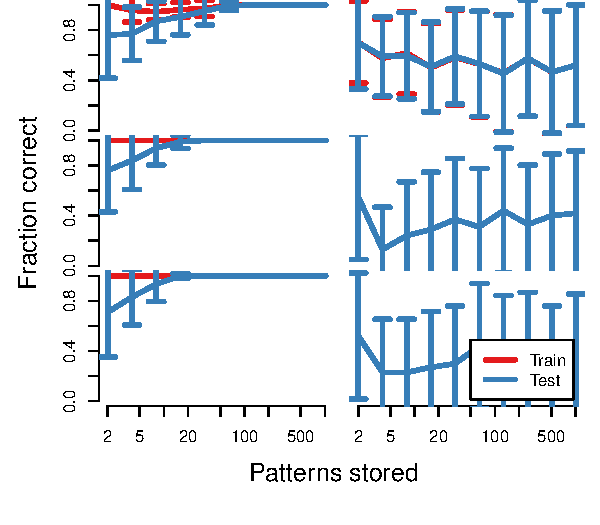
\includegraphics[width=\maxwidth]{../figures/twocolumn-performance-1} 

}

\caption[Performance of pattern recall for select number of patterns, in a perceptron consisting of 10 weights]{Performance of pattern recall for select number of patterns, in a perceptron consisting of 10 weights. The summarisation method is capable of storing nets efficiently, with the hebbian rule performing generally on par with the others, although it is trending towards performing slightly worse when the number of patterns stored is less then the number of nodes. The delta rule with the error input function performs effectivelly equivalently to the perceptron rule as the weights are able to easily adapted regardless of this. The product method performs horribly for all cases, emphasising the linear inseparability that makes the classification difficult.}\label{fig:performance}
\end{figure}
\end{Schunk}

\begin{Schunk}
\begin{figure}[H]

{\centering 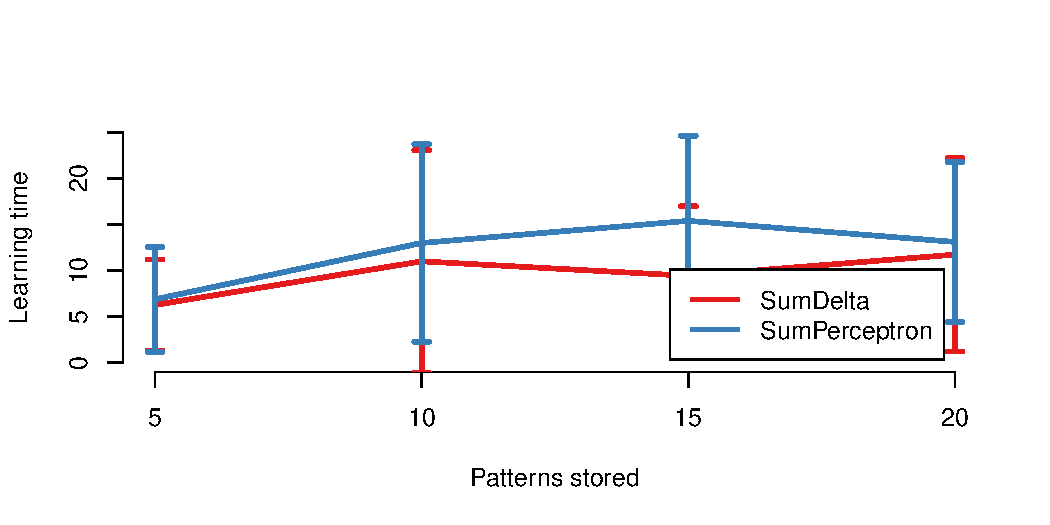
\includegraphics[width=\maxwidth]{../figures/twocolumn-perf_time-1} 

}

\caption[Learning times for the delta and perceptron rule under the summation method for a small range of patterns stored in a 10 node perceptron]{Learning times for the delta and perceptron rule under the summation method for a small range of patterns stored in a 10 node perceptron. Due to the high similarities, the rules perform equivalently. The time here is measured as the number of iterations until all input patterns are recalled correctly.}\label{fig:perf_time}
\end{figure}
\end{Schunk}
	
\paragraph*{3}	
% Multiplicative	




\Cref{fig:3_alignments} shows the orientation of the weight vector under the correlation and covariance rule in the multiplicative and subtractive case, with exemplary randomly assigned initial weights. While it appears to be the case for the correlation method to align to the first principal component of the data, deviating from the mean shows that this is not the case. Further investigations show that it instead aligns to the first eigenvector of the correlation matrix. In contrast, the covariance matrix will by definition have eigenvectors corresponding to the principal components of the data (since the principal components give the vectors with highest variance), and the weight vector will therefore evolve in accordance to that, eventually reaching the stable state of being aligned. 

For the subtractive normalisation with boundaries, the weight vector will evolve according to the eigenvectors of the correlation/covariance matrix minus the average weight change. This will effectively force one weight to steadily increase while the other decreases, meaning that the weights will evolve until on of them hits the boundaries. Consequently, if no action is taken to stop the change for one of the weights while the other hits the boundary, the vector will evolve until the two weights are at either bound, i.e.\ 0 and 1 in our case. 

In \cref{fig:3_initialconditions_mean10}, we can see the final outcome of the simulations based on the initial conditions. For the multiplicative case, the product of the weights are shown, while we in the subtractive case see only where $w_1$ is when any of the weights saturate. We note that we in the multiplicative case clearly have stable fixpoint in aligning to the first PC in most of the cases, but another attractor when the sum of the weights are close to 0. This ought to be because there is an effective division with respect to the sum of the weights, which overthrows the natural development of the weights if causing a large enough shift in relation to the non-diagonality of the correlation matrix. In the covariance case, the difference between the diagonal elements is too small to be noticeable, and we only see the effect when the sum is indeed 0. 


\begin{Schunk}
\begin{figure}[H]

{\centering 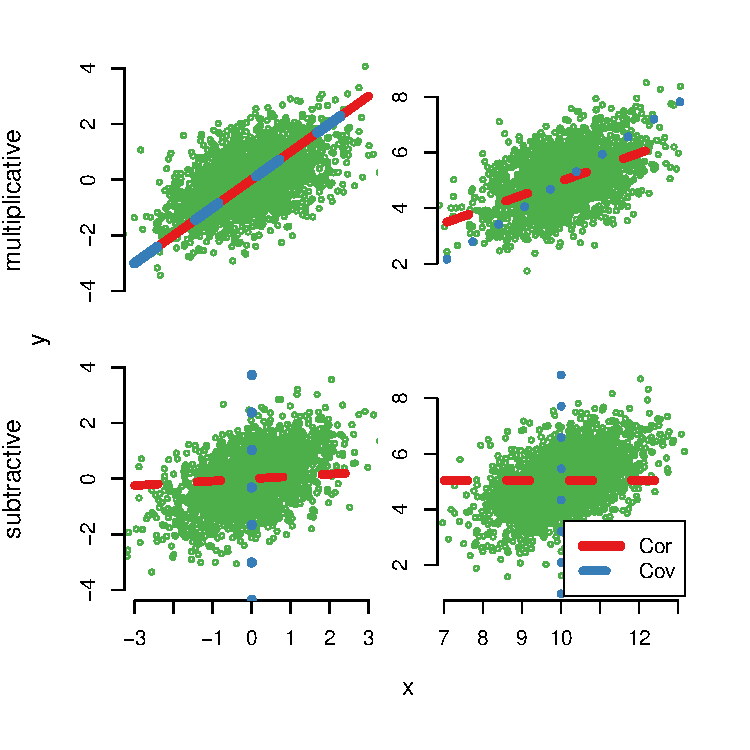
\includegraphics[width=\maxwidth]{../figures/twocolumn-3_alignments-1} 

}

\caption{Final weight vector on top of the data under zero and non-zero circumstances, under both normalisation conditions. Weights initialised randomly. Note how the weight vectors appear to align with the first principal component in the multiplicative case for zero mean.5 Under non-zero mean we do however see how the correlation method aligns to the first eigenvector of the correlation matrix, rather than the principal component of the data. The covariance matrix is nonetheless able to align to the data. Under some circumstances, the vectors align to the second eigenvector (see~\cref{fig:3_initialconditions_mean10}).}\label{fig:3_alignments}
\end{figure}
\end{Schunk}

\begin{Schunk}
\begin{figure}[H]

{\centering 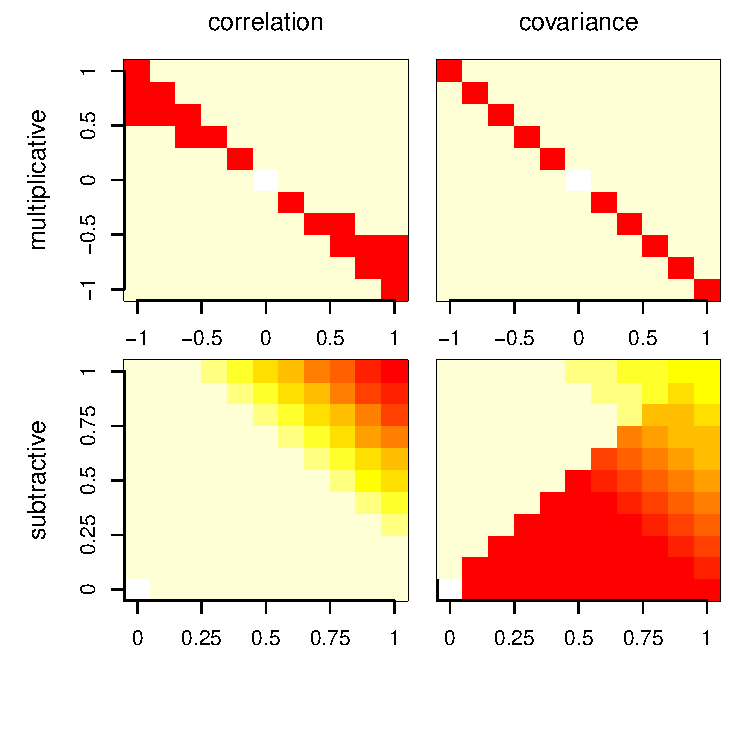
\includegraphics[width=\maxwidth]{../figures/twocolumn-3_initialconditions_mean10-1} 

}

\caption[Outcome dependence on initial conditions when using the correlation method, $x_{mean} = 10$]{Outcome dependence on initial conditions when using the correlation method, $x_{mean} = 10$. The axes represent the initial weights, whereas the colours in the multiplicative case represent the value of the product of the weights, and in the subtractive case simply the value of $w_1$. That is, in the multiplicative case, we get information of which eigenvector of the correlation/covariance matrix the weights have aligned to, while we in the subtractive case simply get information of where the first weight is when the second weight hit a boundary. Under zero mean, the effects will look similar, but the correlation and the covariance case functionally equivalent under multiplicative normalisation, i.e. both with a hard boundary.}\label{fig:3_initialconditions_mean10}
\end{figure}
\end{Schunk}

\Cref{fig:3_weight_devel} shows weight trajectories for most of the interesting cases in \cref{fig:3_initialconditions_mean10}. Wee see in particular how the non-diagonality of the matrices cause different behaviours depending on which weight starts with what value. Even though the ultimate alignment is the same, the weight dynamics are different. The ability of the vectors to align to the principal components will thus depend on the eigenvectors of the matrix governing the updates and the values of the initial weights. Under subtractive normalisation, the weights will only align under \textit{very} improbable conditions. 

\begin{Schunk}
\begin{figure}[H]

{\centering 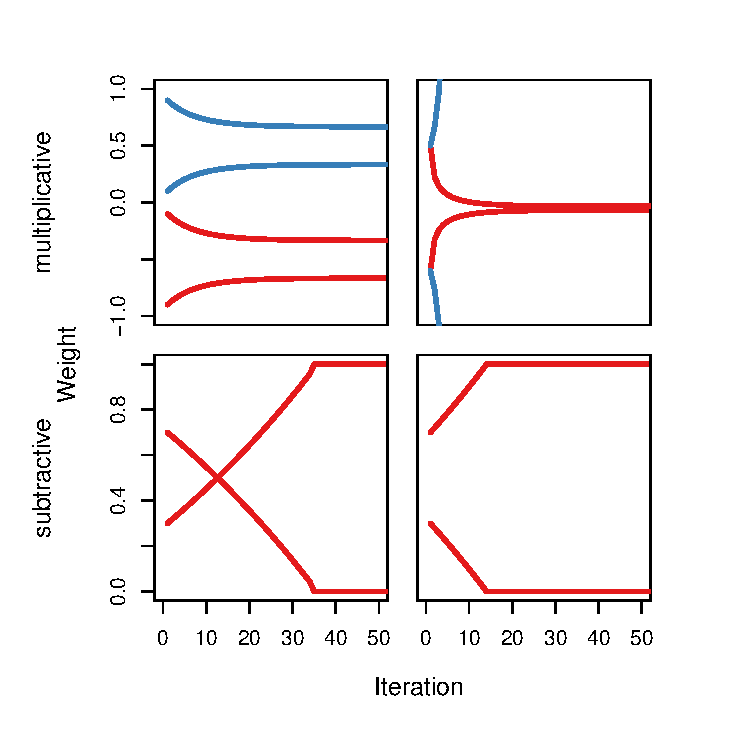
\includegraphics[width=\maxwidth]{../figures/twocolumn-3_weight_devel-1} 

}

\caption{Weight development trajectories for exemplary initial values, corresponding to the different colours in~\cref{fig:3_initialconditions_mean10}. The colours in this figure separates different initial conditions within the same figure. Note how which weight being what changes the dynamics drastically in the multiplicative case when they are of opposite sign, and in the subtractive case when they are of different magnitude.}\label{fig:3_weight_devel}
\end{figure}
\end{Schunk}


\paragraph*{4}




\begin{Schunk}
\begin{figure}[H]

{\centering 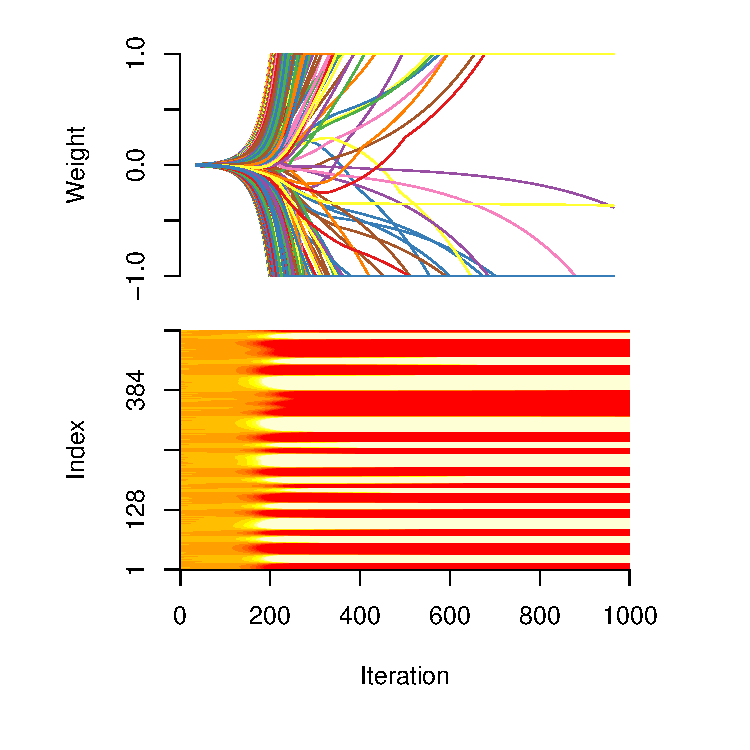
\includegraphics[width=\maxwidth]{../figures/twocolumn-4_ocular_dom-1} 

}

\caption[Ocular dominance patterns driven by weight saturation under subtractive normalisation]{Ocular dominance patterns driven by weight saturation under subtractive normalisation. The upper figure shows the weight trajectories $(w_-)$ for individual cells, whereas the latter shows the same on a map display.}\label{fig:4_ocular_dom}
\end{figure}
\end{Schunk}


\begin{Schunk}
\begin{figure}[H]

{\centering 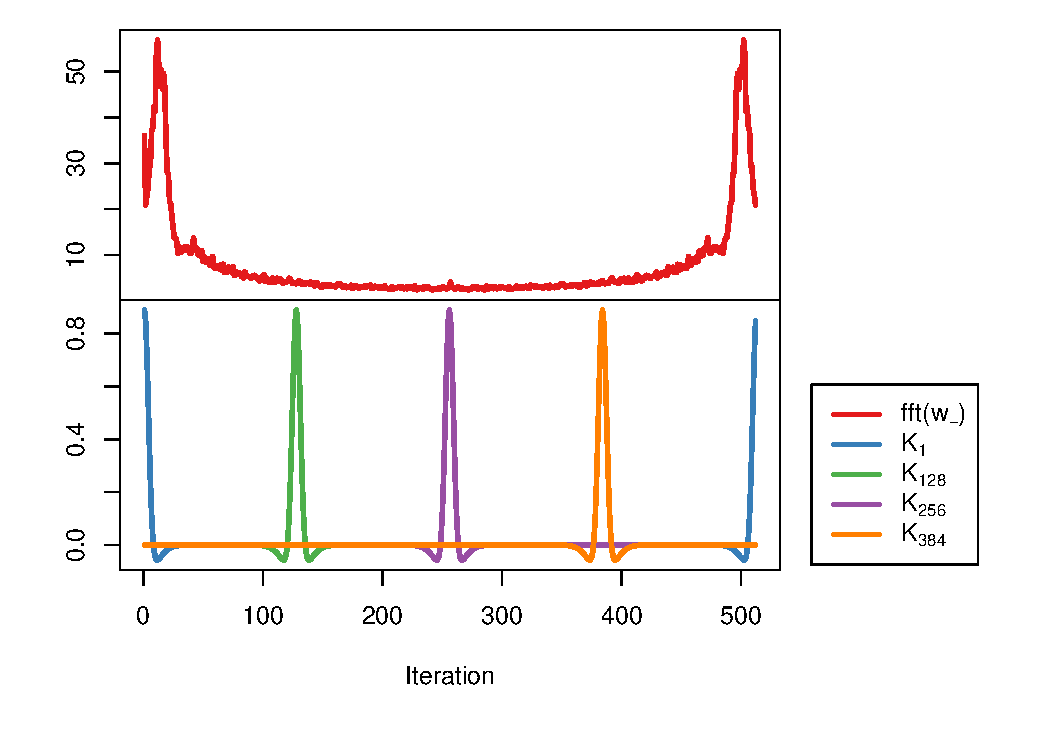
\includegraphics[width=\maxwidth]{../figures/twocolumn-4_Fourier_k-1} 

}

\caption[Upper]{Upper: Fourier transform of the means of the final $w_-$, over 100 simulations. Lower: Individual vectors of the interaction matrix $K$. Note the slightly negative values close to the peaks, showing local competition.}\label{fig:4_Fourier_k}
\end{figure}
\end{Schunk}


\begin{Schunk}
\begin{figure}[H]

{\centering 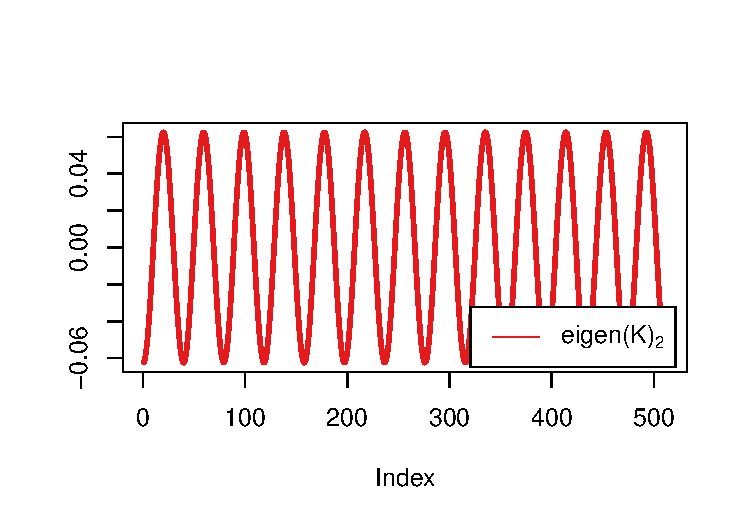
\includegraphics[width=\maxwidth]{../figures/twocolumn-4_K_cos-1} 

}

\caption[Exemplary $K$ eigenvector, showing how the eigenvectors of $K$ correspond to cosinusoidal functions]{Exemplary $K$ eigenvector, showing how the eigenvectors of $K$ correspond to cosinusoidal functions.}\label{fig:4_K_cos}
\end{figure}
\end{Schunk}
Letting the weights be allowed to move freely within the boundaries, we can see how the weights develop in \cref{fig:4_ocular_dom}, where we in the lower part can notice the arisal of the characteristic stripes of ocular dominance.  By changing sigma, i.e.\ the inter-neuronal interaction, we can affect the stripe width as we like. We have removed edge-effects by setting neuron 512 and neuron 1 to be adjacent, and imposing the distance metric under this toroidal landscape. 

\Cref{fig:4_Fourier_k} also shows the mean of the Fourier transforms of the final weights, along with some select rows of the neuronal interaction matrix. The eigenvectors of $K$ will be cosinusoidal functions, which we easily see for example value $K_2$ in \cref{fig:4_K_cos}. Similarly, the eigenvalues give the corresponding frequencies. 


\begin{Schunk}
\begin{figure}[H]

{\centering 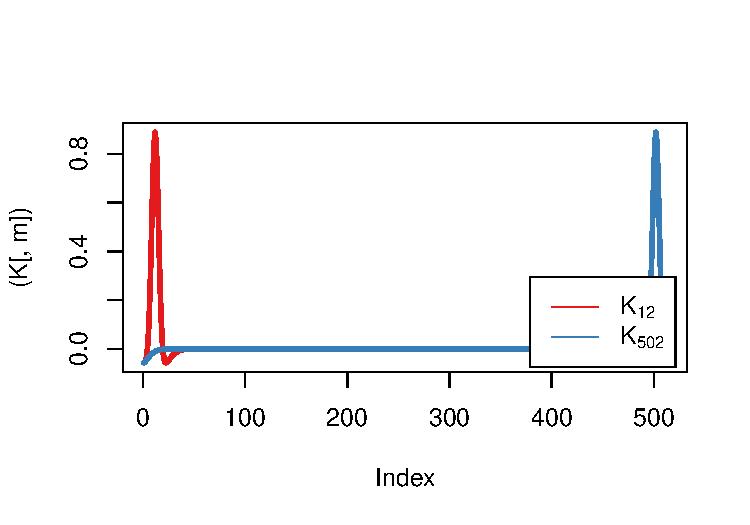
\includegraphics[width=\maxwidth]{../figures/twocolumn-4_max-1} 

}

\caption[The two principal eigenvectors driving the system, first in red, second in blue]{The two principal eigenvectors driving the system, first in red, second in blue. Indices are 12 and 502 respectively.}\label{fig:4_max}
\end{figure}
\end{Schunk}
We also see that the mean of the Fourier transform of the final $w_-$ develops according to the eigenvectors maximizing the Fourier transform of $K$, which we can see by taking the index maximizing the mean Fourier transform of the weights and plotting it, as in \cref{fig:4_max}, where the red curve corresponds to the first PC, and the blue the second.

\section{Acknowledgements}
As always, thanks to Julian Melgar for no particular reason. Also thanks to Olena Yavorska for proving that tidyness trumps compactness.
\bibliography{references}
\end{multicols*}
\newpage
\onecolumn
  \appendix
\section{Code}
   \lstinputlisting{oscillations.R}
   \lstinputlisting{perceptron_perceptron.R}
   \lstinputlisting{unsup_mult.R}
   \lstinputlisting{ocdom.R}
\end{document}
